% flashcards-title: Rectangular tile covered by a grid of unit squares
% flashcards-desc: A rectangle with its longer side marked as four centimeters and its shorter side marked as three centimeters, divided by grid lines into equal small squares. One corner square is shaded, with a note marking it as one centimeter by one centimeter.
\documentclass[dvisvgm,tikz,border=8pt]{standalone}
\usepackage{tikz}
\usetikzlibrary{arrows.meta,calc,positioning}
\definecolor{DeckInk}{HTML}{172A3A}
\definecolor{DeckAccent}{HTML}{176B87}
\definecolor{DeckWarm}{HTML}{D97706}
\definecolor{DeckMuted}{HTML}{667784}
\definecolor{DeckPaper}{HTML}{F7FAFC}
\tikzset{
  every node/.style={font=\sffamily, text=DeckInk},
  object/.style={draw=DeckInk, line width=1.1pt, fill=DeckPaper},
  primary/.style={draw=DeckAccent, line width=1.5pt},
  boundary/.style={draw=DeckAccent, line width=1.5pt, dashed, rounded corners=6pt},
  guide/.style={draw=DeckMuted, line width=0.9pt, dashed},
  dimension/.style={{Stealth[length=3.2mm,width=2.2mm]}-{Stealth[length=3.2mm,width=2.2mm]}, draw=DeckWarm, line width=1.2pt},
  motion/.style={-{Stealth[length=3.5mm,width=2.5mm]}, draw=DeckAccent, line width=1.5pt, dashed},
}

\begin{document}
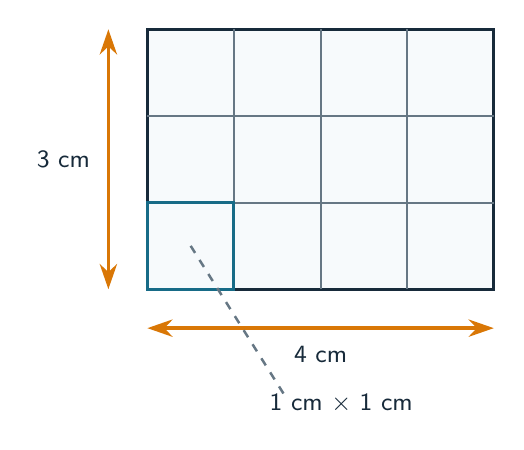
\begin{tikzpicture}[x=1.1cm,y=1.1cm]
  % Shaded unit square in the bottom-left corner
  \fill[DeckAccent!18] (0,0) rectangle (1,1);
  % Tile outline and grid
  \draw[object] (0,0) rectangle (4,3);
  \foreach \i in {1,2,3} \draw[DeckMuted, line width=0.7pt] (\i,0) -- (\i,3);
  \foreach \j in {1,2} \draw[DeckMuted, line width=0.7pt] (0,\j) -- (4,\j);
  \draw[DeckAccent, line width=1.1pt] (0,0) rectangle (1,1);
  % Dimension arrows
  \draw[dimension] (0,-0.45) -- (4,-0.45);
  \node[below, font=\sffamily\small] at (2,-0.55) {4 cm};
  \draw[dimension] (-0.45,0) -- (-0.45,3);
  \node[left, font=\sffamily\small] at (-0.55,1.5) {3 cm};
  % Unit-square note
  \draw[guide] (0.5,0.5) -- (1.6,-1.25);
  \node[below right, font=\sffamily\small, align=left] at (1.3,-1.10) {1 cm $\times$ 1 cm};
\end{tikzpicture}
\end{document}
